\documentclass{beamer}
%
% Josef Hlavac & Tomas Zahradnicky (21.10.2010)
%
%\usepackage{pgfpages}
%\pgfpagesuselayout{4 on 1}[a4paper,border shrink=5mm,landscape]
%\pgfpagesuselayout{resize}[a4paper,border shrink=5mm,landscape]
%\usepackage[czech]{babel}
\usepackage[utf8]{inputenc}
\usepackage{color}
\usepackage{graphicx}
\usepackage{tikz}
\usetikzlibrary{graphs}
\usetikzlibrary{graphs.standard}
\tikzgraphsset{edges={draw,semithick},
nodes={circle,draw,semithick, scale=0.5}}

%\useinnertheme{circles}
\usepackage{subfigure}
\usepackage{minted}
\usepackage{animate}
\usepackage[czech,slovak,english]{babel}%\useinnertheme{rounded}
\usepackage{soul}
%\useinnertheme{rectangles}
%\useinnertheme{balls}
%\usefonttheme{professionalfonts}
%
%\def\uv#1{\char92\relax #1\char34\relax}
%%%%%%%%%%%%%%%%%%%%%%%%%%%%%%%%%%%%%%%%%%%%%%%%%%%%%%%%%%%%%%%%%%
\newcommand\FirstName{Vojtěch}
\newcommand\FirstNameAbbreviated{V}
\newcommand\LastName{Kopal}
\newcommand\Email{kopalvo1@fit.cvut.cz}
\newcommand\Supervisor{Supervisor: Ing.\ Šimon Schierreich}
\newcommand\DissertationTitle{Structural Properties of Sidewalk Netowrks}
\newcommand\Department{Department of Theoretical Computer Science}
%\newcommand\Department{Department of Digital Design}
%\newcommand\Department{Department of Software Engineering}
%\newcommand\Department{Department of Information Security}
\newcommand\Faculty{Faculty of Information Technology}
\newcommand\University{Czech Technical University in Prague}
\newcommand\FacultyAndUniversityAbbr{FIT CTU}
%%%%%%%%%%%%%%%%%%%%%%%%%%%%%%%%%%%%%%%%%%%%%%%%%%%%%%%%%%%%%%%%%%
%\subtitle{BBB}
\subject{SUBJECT}
\author[\FirstNameAbbreviated. \LastName]{\FirstName{} \LastName{} \\{\small \Supervisor}}
\title{\DissertationTitle}
\titlegraphic{
\includegraphics[width=1.5cm]{pic/LogoCVUT.pdf}}
\institute[\FacultyAndUniversityAbbr]{\Department\\ \Faculty\\ \University\\}
\date{June 26, 2024}
%
\begin{document}
\begin{frame}
%\begin{center}
%
\includegraphics[width=1.5cm]{pic/LogoCVUT.pdf}
%\end{center}
\titlepage
\end{frame}

\section{Thesis Goals and Motivation}
\begin{frame}{VBS Blue}
    \begin{figure}
        \centering
        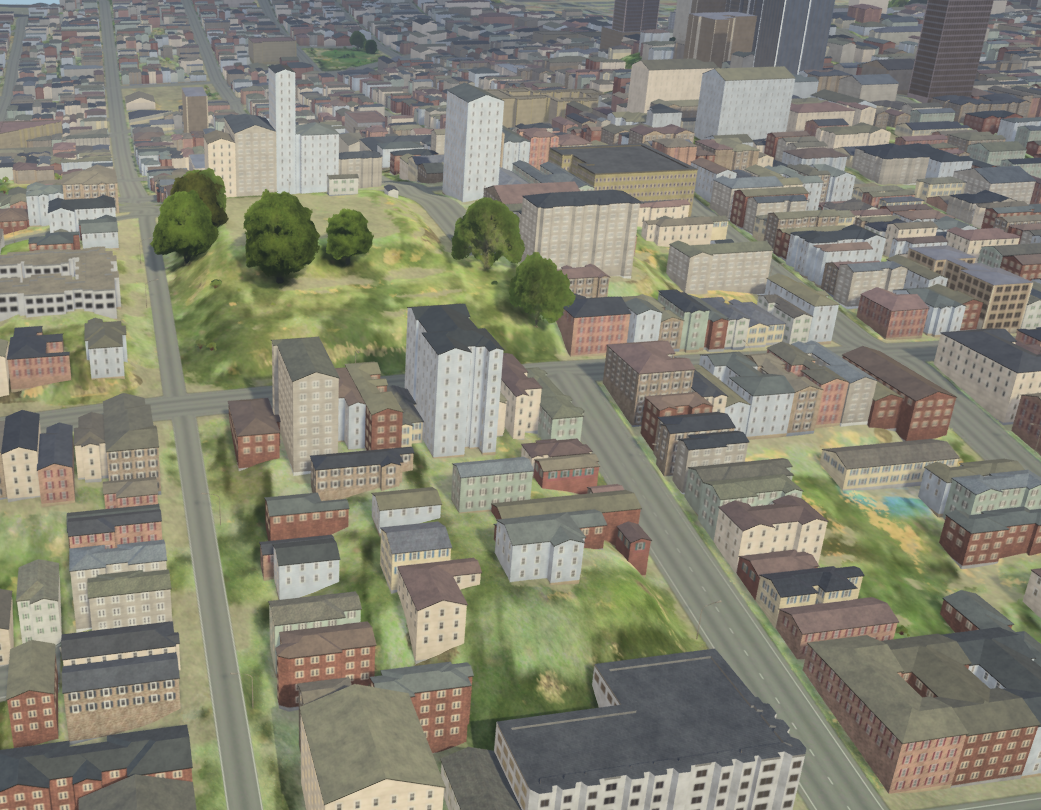
\includegraphics[width=0.75\linewidth]{img/VBSBlue1.png}
        \caption{VBS Blue}
    \end{figure}
\end{frame}

\begin{frame}{VBS Blue}
    \begin{figure}
        \centering
        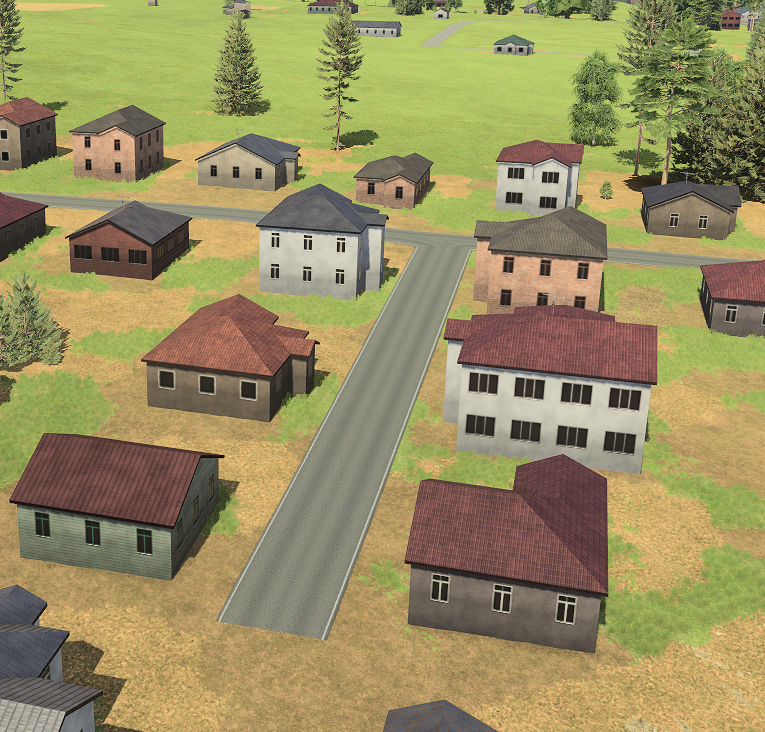
\includegraphics[width=0.7\linewidth]{img/VBSBlue2.png}
        \caption{VBS Blue}
    \end{figure}
\end{frame}

\begin{frame}{Thesis Motivation}

\begin{itemize}
    \item Designing a future algorithm for sidewalk generation
    \item First step – Analysis of the “correct” networks
    \item Properties can be used as
    \begin{itemize} 
        \item Sample data (“correct solution for given part of the world”)
        \item Designing the algorithm so it fits certain property
    \end{itemize}
\end{itemize}


\end{frame}
\begin{frame}{Thesis Goals}

\begin{enumerate}
    \item Obtain the data of real-world sidewalk networks
    \item Measure non-trivial structural properties of these networks 
\end{enumerate}

\end{frame}

\section{Obtaining the Data}
\begin{frame}[fragile]{Obtaining the Data}
    \begin{itemize}
        \item OpenStreetMap data used
        \item Used Python package OSMnx
    \end{itemize}
\end{frame}

\begin{frame}[fragile]{Chosen Locations}
    \begin{itemize}
        \item Černý Most, Prague, Czech Republic
        \item Cēsis, Latvia
        \item College Park, Maryland, United States of America
        \item Dejvice, Prague, Czech Republic
        \item Grenoble, France
        \item Helsinki, Finland
        \item Karlín, Prague, Czech Republic
        \item Raleigh, North Carolina, United States of America
        \item San Sebastián, Spain
        \item Santa Cruz, California, United States of America
    \end{itemize}
\end{frame}

\begin{frame}[fragile, t]{Data Visualization}
    \begin{figure}
        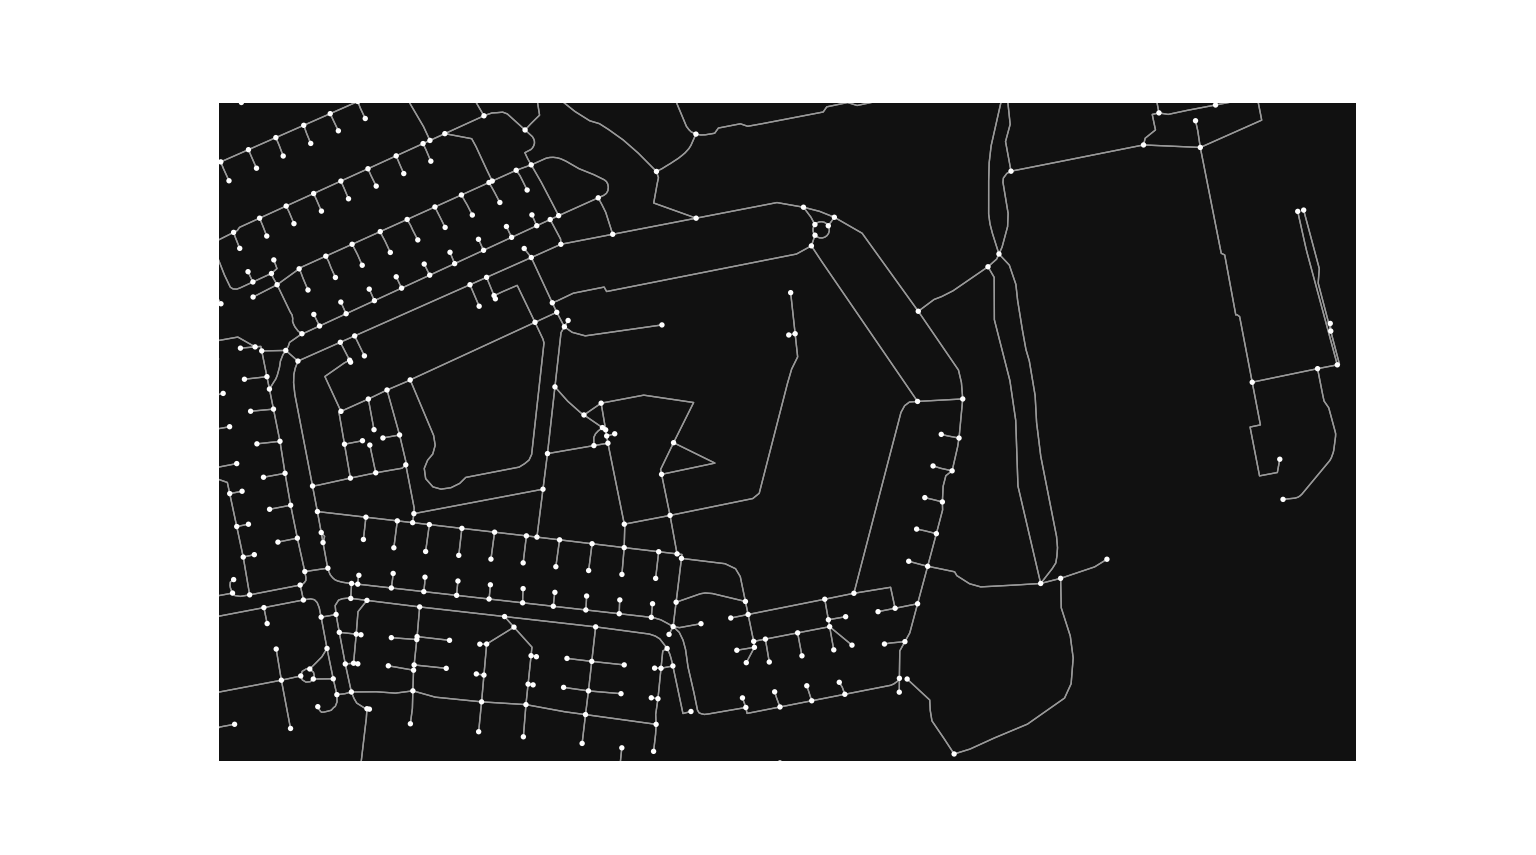
\includegraphics[width=1.0\linewidth]{img/cerny_most_visualization.png}
        \caption{Visualization of sidewalk data for Černý Most}
    \end{figure}
\end{frame}

\section{Properties Measurement}
\begin{frame}{Properties for Measurement}
    \begin{itemize}
        \item Feedback Edge Set Number
        \item Feedback Vertex Set Number
        \item Treewidth
        \item Vertex Cover Number
        \item Edge Cover Number
    \end{itemize}
\end{frame}

\begin{frame}[t]{Feedback Edge Set Number}
    \begin{itemize}
        \item Smallest possible number of edges to remove to create an acyclic graph
        \item Simple measurement by finding MST/MSF
    \end{itemize}
\begin{figure}
    \centering
        \begin{tikzpicture}[every node/.style={draw,circle,very thick}]
        \graph[clockwise, radius=3cm] {subgraph C_n [n=5,name=A] };
        \graph[clockwise, radius=1.5cm] {subgraph I_n [n=5,name=B] };
        
        \foreach \i [evaluate={\j=int(mod(\i+2+4,5)+1)}]% using Paul Gaborit's optimisation
             in {1,2,3,4,5}{
            \draw (A \i) -- (B \i);
            \draw (B \j) -- (B \i);
          }
        \end{tikzpicture}
        \begin{tikzpicture}[every node/.style={draw,circle,very thick}]
          \graph[clockwise, radius=3cm] {subgraph C_n [n=5,name=A] };
          \graph[clockwise, radius=1.5cm] {subgraph I_n [n=5,name=B] };
            \foreach \i [evaluate={\j=int(mod(\i+2+4,5)+1)}]% using Paul Gaborit's optimisation
             in {1,2,3,4,5}{
            \draw (A \i) -- (B \i);
            \draw (B \j) -- (B \i);
            }
            \draw[red] (A 1) -- (B 1);
            \draw[red] (A 1) -- (A 2);
            \draw[red] (A 1) -- (A 5);
            \draw[red] (B 1) -- (B 3);
            \draw[red] (B 1) -- (B 4);
            \draw[red] (A 2) -- (B 2);
            \draw[red] (A 2) -- (A 3);
            \draw[red] (A 5) -- (B 5);
            \draw[red] (A 5) -- (A 4);
        \end{tikzpicture}
        \begin{tikzpicture}[every node/.style={draw,circle,very thick}]
          \graph[clockwise, radius=3cm] {subgraph I_n [n=5,name=A] };
          \graph[clockwise, radius=1.5cm] {subgraph I_n [n=5,name=B] };
            \draw[red] (A 1) -- (B 1);
            \draw[red] (A 1) -- (A 2);
            \draw[red] (A 1) -- (A 5);
            \draw[red] (B 1) -- (B 3);
            \draw[red] (B 1) -- (B 4);
            \draw[red] (A 2) -- (B 2);
            \draw[red] (A 2) -- (A 3);
            \draw[red] (A 5) -- (B 5);
            \draw[red] (A 5) -- (A 4);
        \end{tikzpicture}
        \caption{Feedback Edge Set Number Visualisation on Petersen Graph}
\end{figure}
\end{frame}

\begin{frame}[t]{Feedback Vertex Set Number}
    \begin{itemize}
        \item Smallest possible number of vertices to remove to create an acyclic graph
        \item NP-hard problem
        \item ILP used for finding the lower bound, solver by Yoichi Iwata and Kensuke Imanishi for upper bound
    \end{itemize}
\begin{figure}
    \centering
        \begin{tikzpicture}[every node/.style={draw,circle,very thick}]
          \graph[clockwise, radius=3cm] {subgraph C_n [n=5,name=A] };
          \graph[clockwise, radius=1.5cm] {subgraph I_n [n=5,name=B] };
        
          \foreach \i [evaluate={\j=int(mod(\i+2+4,5)+1)}]% using Paul Gaborit's optimisation
             in {1,2,3,4,5}{
            \draw (A \i) -- (B \i);
            \draw (B \j) -- (B \i);
          }
        \end{tikzpicture}
        \begin{tikzpicture}[every node/.style={draw,circle,very thick}]
            \graph[clockwise, radius=3cm] {subgraph C_n [n=5,name=A] };
            \graph[clockwise, radius=1.5cm] {subgraph I_n [n=5,name=B] };
            
            \foreach \i [evaluate={\j=int(mod(\i+2+4,5)+1)}] in {1,2,3,4,5}{
                    \draw (A \i) -- (B \i);
                    \draw (B \j) -- (B \i);
                }
            \node[draw,circle,very thick,red,scale=0.5] at (A 5) {5};
            \node[draw,circle,very thick,red,scale=0.5] at (B 3) {3};
            \node[draw,circle,very thick,red,scale=0.5] at (B 4) {4};
        \end{tikzpicture}
        \begin{tikzpicture}[every node/.style={draw,circle,very thick}]
            \graph[clockwise, radius=3cm] {subgraph C_n [n=5,name=A] };
            \graph[clockwise, radius=1.5cm] {subgraph I_n [n=5,name=B] };
            
            \foreach \i [evaluate={\j=int(mod(\i+2+4,5)+1)}] in {1,2,3,4,5}{
                \draw (A \i) -- (B \i);
                \draw (B \j) -- (B \i);
            }
            \node[draw,circle,very thick,white,scale=0.5] at (A 5) {5};
            \node[draw,circle,very thick,white,scale=0.5] at (B 3) {3};
            \node[draw,circle,very thick,white,scale=0.5] at (B 4) {4};
            
            \draw[white] (A 1) -- (A 5);
            \draw[white] (A 4) -- (A 5);
            \draw[white] (B 5) -- (A 5);
            \draw[white] (A 4) -- (B 4);
            \draw[white] (B 1) -- (B 4);
            \draw[white] (B 2) -- (B 4);
            \draw[white] (B 1) -- (B 3);
            \draw[white] (B 5) -- (B 3);
        \end{tikzpicture}
    \caption{Visualization of Feedback Vertex Set Number on Petersen Graph}
\end{figure}
\end{frame}
\begin{frame}[t]{Treewidth}
    \begin{itemize}
        \item Algorithmic distance of the given graph to a tree using a tree decomposition
        \item NP-hard problem
        \item Used twalgor solver developed by Hisao Tamaki
    \end{itemize}
    \begin{figure}
        \centering
        \begin{tikzpicture}[every node/.style={draw,circle,very thick}]
          \graph[clockwise, radius=3cm] {subgraph C_n [n=5,name=A] };
          \graph[clockwise, radius=1.5cm] {subgraph I_n [n=5,name=B] };
        
          \foreach \i [evaluate={\j=int(mod(\i+2+4,5)+1)}]% using Paul Gaborit's optimisation
             in {1,2,3,4,5}{
            \draw (A \i) -- (B \i);
            \draw (B \j) -- (B \i);
          }
        \end{tikzpicture}
        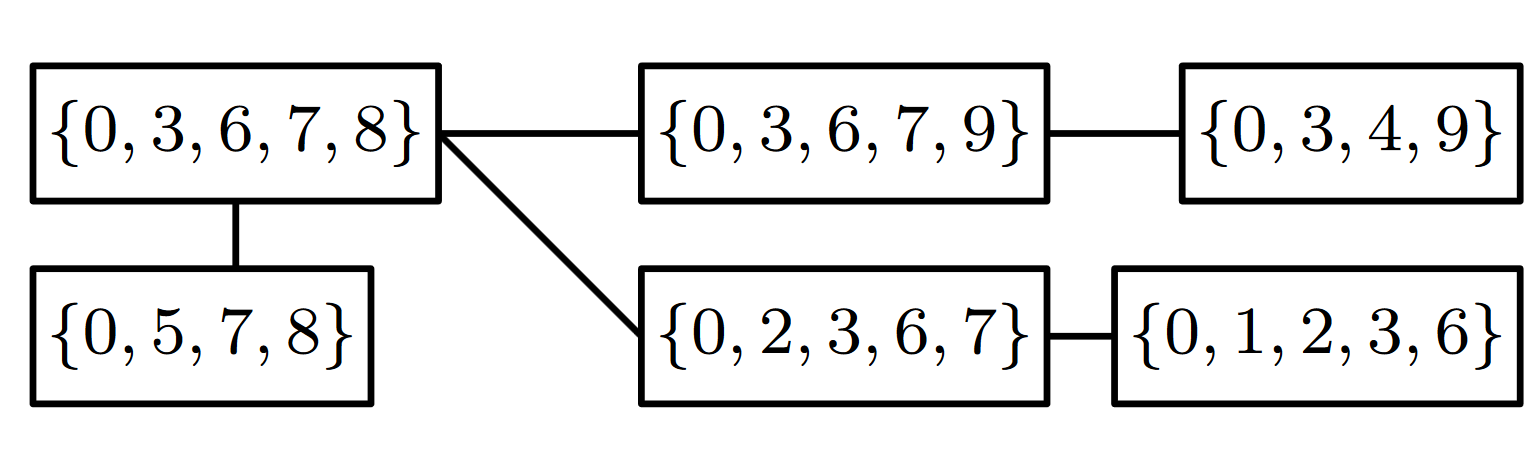
\includegraphics[width=0.5\linewidth]{img/petersen_tree_decomposition.png}
        \caption{Optimal Tree Decomposition of Petersen Graph}
    \end{figure}
\end{frame}

\begin{frame}[t]{Vertex Cover Number}
    \begin{itemize}
        \item Minimal subset of vertices, such that every edge is incident with at least one vertex in the subset
        \item Solved using ILP (NP-hard problem)
    \end{itemize}
    \begin{figure}
        \begin{tikzpicture}[every node/.style={draw,circle,very thick}]
          \graph[clockwise, radius=3cm] {subgraph C_n [n=5,name=A] };
          \graph[clockwise, radius=1.5cm] {subgraph I_n [n=5,name=B] };
        
          \foreach \i [evaluate={\j=int(mod(\i+2+4,5)+1)}]% using Paul Gaborit's optimisation
             in {1,2,3,4,5}{
            \draw (A \i) -- (B \i);
            \draw (B \j) -- (B \i);
          }
        \end{tikzpicture}
        \begin{tikzpicture}[every node/.style={draw,circle,very thick}]
                \graph[clockwise, radius=3cm] {subgraph C_n [n=5,name=A] };
                \graph[clockwise, radius=1.5cm] {subgraph I_n [n=5,name=B] };
            
                \foreach \i [evaluate={\j=int(mod(\i+2+4,5)+1)}] in {1,2,3,4,5}{
                    \draw (A \i) -- (B \i);
                    \draw (B \j) -- (B \i);
                }
                \node[draw,circle,very thick,red,scale=0.5] at (A 1) {1};
                \node[draw,circle,very thick,red,scale=0.5] at (A 2) {2};
                \node[draw,circle,very thick,red,scale=0.5] at (A 4) {4};

                \node[draw,circle,very thick,red,scale=0.5] at (B 3) {3};
                \node[draw,circle,very thick,red,scale=0.5] at (B 4) {4};
                \node[draw,circle,very thick,red,scale=0.5] at (B 5) {5};
            \end{tikzpicture}
            \caption{Optimal Vertex Cover of Petersen Graph}
    \end{figure}
\end{frame}

\begin{frame}[t]{Edge Cover Number}
    \begin{itemize}
        \item Minimal subset of edges, such that every vertex is contained in at least one edge in the subset
        \item Solved using ILP
    \end{itemize}
    \begin{figure}
        \begin{tikzpicture}[every node/.style={draw,circle,very thick}]
          \graph[clockwise, radius=3cm] {subgraph C_n [n=5,name=A] };
          \graph[clockwise, radius=1.5cm] {subgraph I_n [n=5,name=B] };
        
          \foreach \i [evaluate={\j=int(mod(\i+2+4,5)+1)}]% using Paul Gaborit's optimisation
             in {1,2,3,4,5}{
            \draw (A \i) -- (B \i);
            \draw (B \j) -- (B \i);
          }
        \end{tikzpicture}
                    \begin{tikzpicture}[every node/.style={draw,circle,very thick}]
                \graph[clockwise, radius=3cm] {subgraph C_n [n=5,name=A] };
                \graph[clockwise, radius=1.5cm] {subgraph I_n [n=5,name=B] };
            
                \foreach \i [evaluate={\j=int(mod(\i+2+4,5)+1)}] in {1,2,3,4,5}{
                    \draw[red] (A \i) -- (B \i);
                    \draw (B \j) -- (B \i);
                }
            \end{tikzpicture}
            \caption{Optimal Edge Cover of Petersen Graph}
    \end{figure}
\end{frame}

\begin{frame}[t]{Results}
\begin{table}[h!]
\centering
\resizebox{\textwidth}{!}{%
\begin{tabular}{l|c|c|c|c|c|c|c}
	\textbf{Dataset}		& $\|\mathbf{V}\|$		& $\|\mathbf{E}\|$& \textbf{FESN}   & \textbf{FVSN}    & \textbf{TW}  & \textbf{VCN}  &   \textbf{ECN} \tabularnewline \hline \hline
 	Černý Most, PRG, CZE & 1\,553	& 1\,893 & 377 & 146--167 & 10  &   764 &   806\tabularnewline \hline
 	Cēsis, LAT	& 1\,122	& 1\,244	& 245 & 110--113 & 10    &   521 &   606 \tabularnewline \hline
 	College Park, MD, USA & 5\,110 & 6\,392 & 1\,534 & 571--595	 & 15--22 &   2\,440    &   2\,725\tabularnewline \hline
 	Dejvice, PRG, CZE & 1\,675 & 1\,907 & 372 & 173	 & 9  &   790 &   900\tabularnewline \hline
 	Grenoble, FRA & 9\,647 & 11\,688 & 2\,711 & 1\,017--  & 14--25    &   4\,672  &   5\,093\tabularnewline \hline
    Helsinki, FIN & 115\,318 & 123\,291 & 18\,483 & 7\,842--    &    & 52\,824  &   63\,343\tabularnewline \hline
 	Karlín, PRG, CZE & 1\,070 & 1\,364 & 345 & 138--153 & 8   &   535 &   549\tabularnewline \hline
 	Raleigh, NC, USA & 36\,385 & 39\,930 & 5\,667 & 2\,472--	& & 16\,576  &   19\,942\tabularnewline \hline
 	San Sebastián, ESP & 4\,782 & 4\,961 & 813 & 407	 & 7 &   2\,173  &   2\,639\tabularnewline \hline
 	Santa Cruz, CA, USA & 13\,060 & 14\,494 & 2\,710 & 1\,168--   &   13--16  &   6\,059	 & 7\,135\tabularnewline
\end{tabular}}
\caption[Concluding table]{~Measured values of all parameters.}\label{tab:all}
\end{table}
\end{frame}

\section{Questions}
\begin{frame}{Data Quality Assurance}
    \begin{itemize}
        \item Locations were picked based on the presence of sidewalk data in OpenStreetMap
        \item Data were checked mainly for the missing parts, rather than the superfluous data
        \item The data were mainly checked on the level of visualization than on the graph level
    \end{itemize}
\end{frame}

\begin{frame}{Selection of Properties}
    \begin{itemize}
        \item Selected properties that could be handy for future algorithm, or could be academically interesting
        \item All properties, apart from edge cover number, were mentioned in the assignment
        \item I have added the edge cover number as I wanted another parameter computable in polynomial time
    \end{itemize}
\end{frame}

\begin{frame}{Are the Values of Edge Cover Number Low?}
    \begin{itemize}
        \item Edge cover number, for a graph of $n$ vertices, will be equal to a natural number $e$, where $\left \lceil{\frac{n}{2}}\right \rceil  \leq e \leq n - 1$
        \item The values may not be nominally low, but relatively to the graph size, the number is low, as it falls always in the bottom 11 \% of possible values in all cases
    \end{itemize}
\begin{table}[h!]
\centering
\resizebox{\textwidth}{!}{%
\begin{tabular}{l|c|c|c|c|c|c}
	\textbf{Dataset}		& $\|\mathbf{V}\|$		& $\|\mathbf{E}\|$& \textbf{ECN}   & \textbf{Minimal}    & \textbf{Maximal}  & \textbf{Percentile} \tabularnewline \hline \hline
 	Černý Most, PRG, CZE & 1\,553	& 1\,893 & 806 & 777 & 1\,552  &   3.74 \%\tabularnewline \hline
 	Cēsis, LAT	& 1\,122	& 1\,244	& 606 & 561 & 1121    &   8.04 \% \tabularnewline \hline
 	College Park, MD, USA & 5\,110 & 6\,392 & 2\,725 & 2\,555 & 5\,109 &   6.66 \%\tabularnewline \hline
 	Dejvice, PRG, CZE & 1\,675 & 1\,907 & 900 & 838	 & 1\,674  &   7.42 \% \tabularnewline \hline
 	Grenoble, FRA & 9\,647 & 11\,688 & 5\,093 & 4\,824  & 9\,646    &   5.58 \%   \tabularnewline \hline
    Helsinki, FIN & 115\,318 & 123\,291 & 63\,343 & 57\,659    &  115\,317  & 9.89 \% \tabularnewline \hline
 	Karlín, PRG, CZE & 1\,070 & 1\,364 & 549 & 535 & 1\,069   &   0.26 \%\tabularnewline \hline
 	Raleigh, NC, USA & 36\,385 & 39\,930 & 19\,942 & 18\,193	& 36\,384 & 9.61 \%  \tabularnewline \hline
 	San Sebastián, ESP & 4\,782 & 4\,961 & 2\,639 & 2\,391	 & 4\,781 &   10.38 \%    \tabularnewline \hline
 	Santa Cruz, CA, USA & 13\,060 & 14\,494 & 7\,135 & 6\,530   &   13\,059  &   9.27 \%	 \tabularnewline
\end{tabular}}
\end{table}
\end{frame}

\begin{frame}{Error with Simple Loops}
    \begin{itemize}
        \item There was an inconsistency in counting simple loops (edges starting and ending in the same vertex) in the graphs between measured properties
        \item Number of loops in graphs is relatively small, therefore the main takeaways from the measurements are still valid
    \end{itemize}
    \begin{table}
    \begin{tabular}{l|c|c}
	\textbf{Dataset} & $\|\mathbf{E}\|$& Number of Loops  \tabularnewline \hline \hline
 	Černý Most, PRG, CZE & 1\,893 & 2 \tabularnewline \hline
 	Cēsis, LAT	& 1\,244	& 3 \tabularnewline \hline
 	College Park, MD, USA & 6\,392 & 6 \tabularnewline \hline
 	Dejvice, PRG, CZE & 1\,907 & 6 \tabularnewline \hline
 	Grenoble, FRA & 11\,688 & 21  \tabularnewline \hline
    Helsinki, FIN & 123\,291 & 159 \tabularnewline \hline
 	Karlín, PRG, CZE & 1\,364 & 3 \tabularnewline \hline
 	Raleigh, NC, USA & 39\,930 & 59 \tabularnewline \hline
 	San Sebastián, ESP & 4\,961 & 11 \tabularnewline \hline
 	Santa Cruz, CA, USA  & 14\,494 &60 \tabularnewline
  \end{tabular}
  \end{table}
\end{frame}

\begin{frame}{Used Scripts and Data}
    \begin{itemize}
        \item Made publicly available on \url{https://github.com/VojtechKopal/StructuralPropertiesOfSidewalkNetworks}
    \end{itemize}
\end{frame}

\end{document}
